\documentclass[11pt,a4paper]{article}
\usepackage{tabularx}
\usepackage{ltablex}
\usepackage{graphicx}
\usepackage{tabularx}
\usepackage[cache=false]{minted}
\setminted[erlang]{
frame=lines,
framesep=2mm,
baselinestretch=1.1,
fontsize=\footnotesize,
linenos,
breaklines}
\setminted[python]{
frame=lines,
framesep=2mm,
baselinestretch=1.1,
fontsize=\footnotesize,
linenos,
breaklines}
\setminted[bnf]{
frame=lines,
framesep=2mm,
baselinestretch=1.1,
fontsize=\footnotesize,
linenos,
breaklines}
\usemintedstyle{friendly}
% Add Subtitle
\usepackage{titling}
\newcommand{\subtitle}[1]{%
  \posttitle{%
    \par\end{center}
    \begin{center}\large#1\end{center}
    \vskip0.5em}%
}

\begin{document}

\title{Web Science Exam 2019}

\author{Username: zlp432}
\date{\today}
	
\maketitle
\tableofcontents

\section{WWW as a network and challenges}

Since the world wide web is a very big collection of data there will be lots of problems with duplications or even spamming (wrong information).
Also the data on the web can pretty much change at any time which makes it hard to keep up with all changes. 
The format is also a problem, which needs to be taken care of, mostly HTML which then has to be processed that really only the important content is left.


\section{Recommender systems}

\subsection{Question 1}
I used the \texttt{surprise} library for the collaborative filtering part.
In the code I decided to use \texttt{SVD} for building a recommendation model + KNN as a comparison to it and calculated the RMSE according to it.
I also thought of implementing both item/user based approach as well but left it then since the Matrix factorization approach seemed good enough of an example.

\subsection{Question 2}
I ended up using \texttt{n-grams=3} (for genres), so recommendations will be done according to the

\subsection{Question 3}

\subsection{Question 4}
A possible solution to that would be just the movies which have the highest ratings, or movies which have been rated highly by the most people.
Since if the majority likes the movies then with some probability also the new user will like them.
But in this case there is not much information to get from our dataset, so either the user would need to provide some information (favourite movie, genres he likes), or we can only give recommendations according to what the majority likes or thinks is a good movie.
Or we could even go as far as just getting randomized movies (a sample), from which maybe any is a movie the user actually likes, and then start from there and take into account what kind of movies he is actually watching.

\subsection{Question 5}

The collaborative filtering solution is in my opinion also ok for bigger datasets since I build a model which then can be reused for as much data as needed (can of course also be retrained with more data).
The content recommender on the other hand needs to calculate TF-IDF vectors before calculating the cosinus simularity between all the movies according to genre, which isn't too great if it keeps needing to recalculate it.
So here would be model based approach much better then the memory based approach.


\section{Sentiment and data mining}

\subsection{Task 1}
As far as I understood the task I created the tokes by using the \texttt{CountVectorizer} with n-gram=2 to create all the bi-grams for each review.
Additionally to that I then Transformed those tokens into TF-IDF (which tells me the term frequency etc.) which I then used to train my model.
I preprocess the reviews with stemming, removing stop words, lower all texts and especially remove HTML tags ($<br /> ->$ new lines).
This way I can reduce for once tokens which would be useless (HTML tags, punctuations), as well as with stemmed words I hope to find find better matches (reducing to word stem), which should end in better predictions in the end.


\subsection{Task 2}
I tried a few classifiers but in the end I decided to go with \texttt{MultinomialNB}(Multinominal Naive Basis), which is a very basic Classification but has a good enough accuracy for this task in my opinion.
I also wanted to train a \texttt{RandomForrest} Model but that just took forever, so I ended up with a Naive Basis model.
On the Naive Basis classifier I also run a \texttt{GridSearchCV} on my classifier to try to improve my parameters a little to get a better accuracy, even though in the end it's only a marginal improvement.



\subsection{Task 3}

For this task I used the library \texttt{lime} to help me, because it visualizes very nicely why a review has been wrongly classified according to which words.
For that I chose 5 randomly not rightly classified reviews out of the test data.

So for the classes \mintinline{python}{{'positive': 1, 'negative' 0}} I get the following false classified reviews:

\newpage
\subsubsection{Review 1}
\begin{tabularx}{\textwidth}{l|X|X}
\textbf{ID} & \textbf{Original Text} & \textbf{Preprocessed Text}\\
\hline
7894 &
In this film I prefer Deacon Frost. He\'s so sexy! I love his glacial eyes! I like Stephen Dorff and the vampires, so I went to see it. I hope to see a gothic film with him. "Blade" it was very "about the future". If vampires had been real, I would be turned by Frost!
&
film prefer deacon frost he sexi love glacial eye like stephen dorff vampir went see hope see gothic film blade futur vampir real would turn frost
\end{tabularx}

\begin{figure}[htb!]
	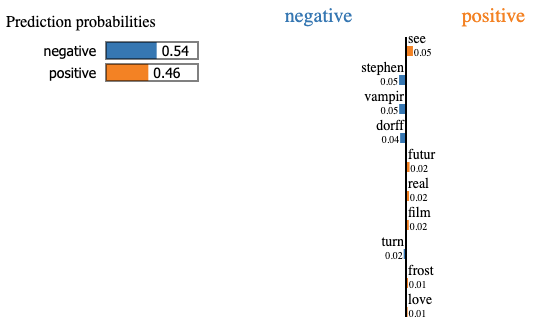
\includegraphics[width=\textwidth]{img/review_1}
	\caption{Wrongly classified review 1}
\end{figure}
\textbf{Reasons for wrong classification:}

As we see here in the original there was talk about vampires which is seen as a negative thing (which technically is true for horror movies etc.),but in this case it was actually a positive review but the positive words don't outweigh the negative ones.
So that the review got wrongly classified as negative

\newpage
\subsubsection{Review 2}
\begin{tabularx}{\textwidth}{l|X|X}
\textbf{ID} & \textbf{Original Text} & \textbf{Preprocessed Text}\\
\hline
8108 &
This movie is such a fine example of the greatness that is 80's entertainment. Oh don't get me wrong, most of the music back then sucked. I only ever liked the metal bands from the 80s. Bands that had some balls. Forget that whiny keyboard crap and all that 'life is horrible and I want to die' garbage. But the movies from the 80's are the best. They were all about nonsense and just having a good time. This movie exemplifies that! Party! Get naked! Get laid! WOOOOOOHOOOOO!
&
movi fine exampl great 80 entertain oh dont get wrong music back suck ever like metal band 80 band ball forget whini keyboard crap life horribl want die garbag movi 80 best nonsens good time movi exemplifi parti get nake get laid woooooohooooo
\end{tabularx}

\begin{figure}[htb!]
	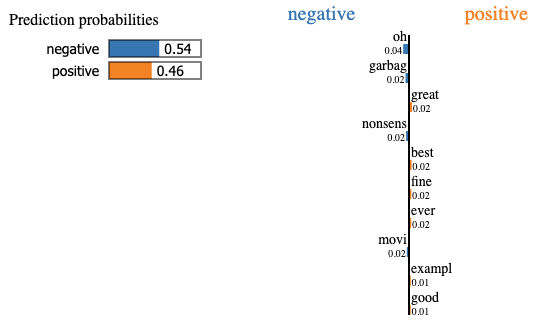
\includegraphics[width=\textwidth]{img/review_2}
	\caption{Wrongly classified review 2}
\end{figure}

\textbf{Reasons for wrong classification:}

Also here again negative words outweigh, positive ones. But in that example "oh" is weighted quite high.
So also an example again of a too high weighted negative words in comparison to positive ones.

\newpage
\subsubsection{Review 3}

\begin{tabularx}{\textwidth}{l|X|X}
\textbf{ID} & \textbf{Original Text} & \textbf{Preprocessed Text}\\
\hline
8205 & 
Agreeable "Boy's Own Paper" nonsense with a sprightly performance from Cushing, some amusing rubber monsters, colourful jungle sets, \& the ever-welcome appearance of Caroline Munro in animal skins.
&
agreeabl boy paper nonsens sprightli perform cush amus rubber monster colour jungl set ever welcom appear carolin munro anim skin
\end{tabularx}

\begin{figure}[htb!]
	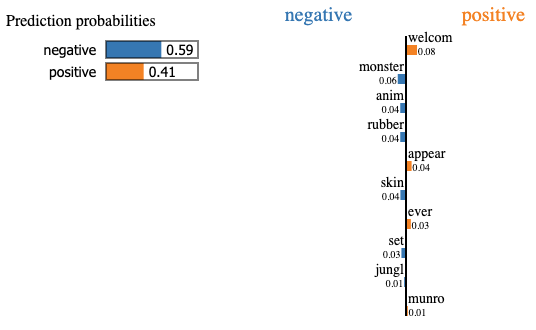
\includegraphics[width=\textwidth]{img/review_3}
	\caption{Wrongly classified review 3}
\end{figure}

\textbf{Reasons for wrong classification:}
Also again words which are seen as more negative like "monsters" or "rubber" etc. don't really help in seeing an actual positive review in it.

\newpage
\subsubsection{Review 4}
\begin{tabularx}{\textwidth}{l|X|X}
\textbf{ID} & \textbf{Original Text} & \textbf{Preprocessed Text}\\
\hline
21196 &
It's dreadful, but ...$<br /><br />$Cat Stevens fans are given the opportunity to see the woman who inspired the lovely song "Lady D'Arbanville" on his album "Mona Bone Jakon", before Cat turned into a fatwa-supporting religious zealot.
&
dread cat steven fan given opportun see woman inspir love song ladi darbanvil album mona bone jakon cat turn fatwa support religi zealot
\end{tabularx}

\begin{figure}[htb!]
	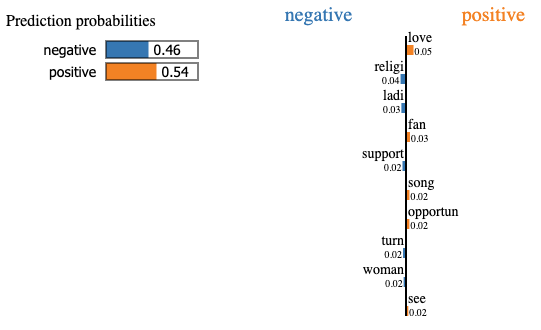
\includegraphics[width=\textwidth]{img/review_4}
	\caption{Wrongly classified review 4}
\end{figure}

\textbf{Reasons for wrong classification:}
Here also a more positive talk about Cat Stevens first but actually meant in a negative way, so easily can be misinterpreted as a positive review instead of a negative one.


\newpage
\subsubsection{Review 5}
\begin{tabularx}{\textwidth}{l|X|X}
\textbf{ID} & \textbf{Original Text} & \textbf{Preprocessed Text}\\
\hline
23262 &
I was pleasantly surprised with this one. It's actually quite interesting and engaging. The cast is strong, even Dan Cortese. Brooke Shields has come into her own as an actress. Black and White must have really set her free, 'cause I have never seen her in this much command playing a conventional character. If marketed right, could be a medium-size hit.
&
pleasantli surpris one actual quit interest engag cast strong even dan cortes brook shield come actress black white must realli set free caus never seen much command play convent charact market right could medium size hit
\end{tabularx}

\begin{figure}[htb!]
	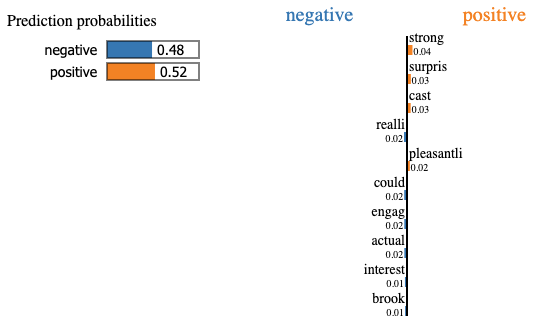
\includegraphics[width=\textwidth]{img/review_5}
	\caption{Wrongly classified review 5}
\end{figure}

\textbf{Reasons for wrong classification:}
Also here lots of positive words like "engaging" etc. but actually meant as a negative review "medium-size hit", but also here hard to distinguish again since many positive words have been used.




\end{document}